\newpage
\chapter{Hasil dan Pembahasan} \label{Bab IV}

\section{Hasil Penelitian} \label{IV.Hasil}
Berisi hasil penelitian berdasarkan rancangan yang sudah dijelaskan pada Bab \ref{Bab III}, terutama dari Subbab \ref{III.Metode}. Bagi yang membuat alat, jelaskan alat yang jadi dalam bentuk apa. Bagi yang membuat aplikasi, jelaskan aplikasi yang jadi dalam bentuk seperti apa. Jabarkan dalam bentuk pseudocode dan dijelaskan per bagian kodenya. Gunakan gambar dan tabel sebagai alat bantu menjelaskan hasil. \par

\section{Hasil Pengujian} \label{IV.Uji}
Berikan hasil pengujian berdasarkan rancangan \& skenario yang sudah direncanakan sebelumnya pada Subbab \ref{III.Rancang Uji}. \par

\begin{longtable}{|c|c|c|}
	\caption{Contoh Hasil Pengujian}
	\label{table:4.uji}\\
	\hline
	\textbf{Pengujian} & \textbf{Metode A} & \textbf{Metode B} \\
	\hline
	\endhead
	Kecepatan & 10 ms & 12 ms \\ 
	\hline
	Memori & 10 MB & 7 MB \\
	\hline
\end{longtable}

\begin{figure}[H]
	\centering
	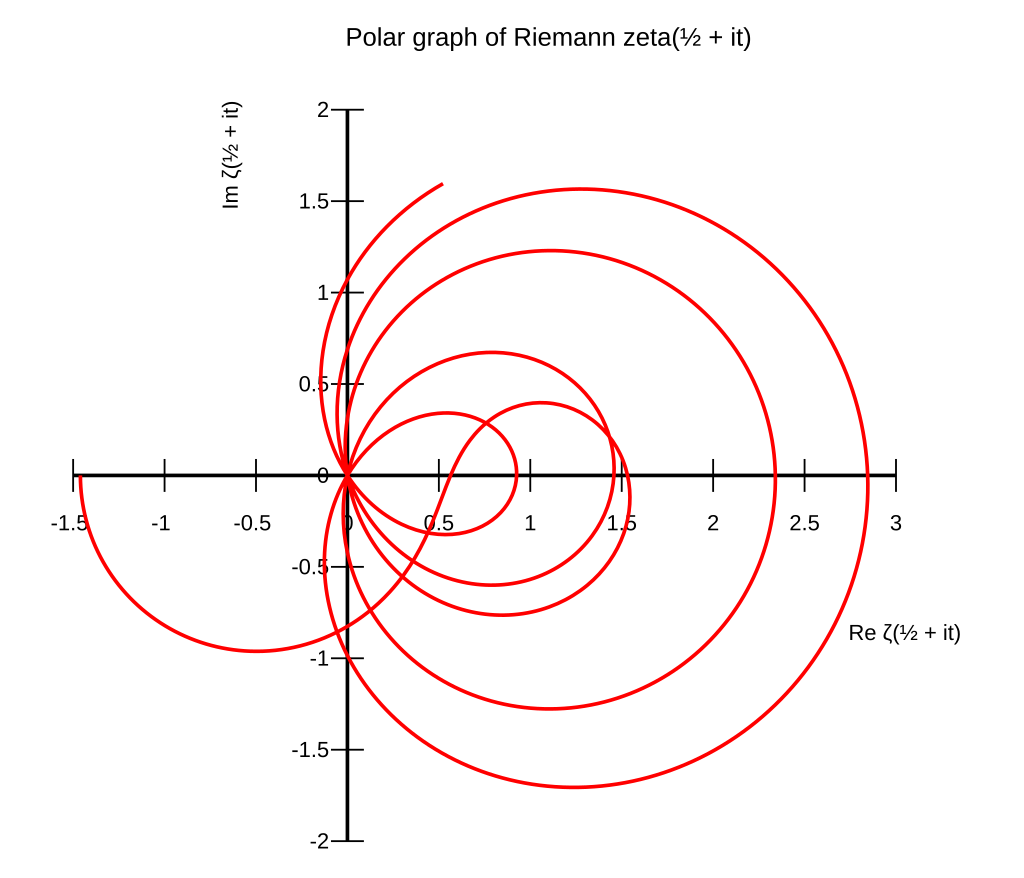
\includegraphics[width=0.5\textwidth]{figure/zeta.png}
	\caption{Contoh Graf Pengujian}
	\label{fig:4.graf}
\end{figure}

\section{Analisis Hasil Penelitian} \label{IV.Analisis}
Berikan analisis hasil penelitian \& pengujian, berupa data yang didapatkan dari penelitian \& pengujian Tugas Akhir yang sudah anda kerjakan. Gunakan gambar dan tabel sebagai alat bantu menjelaskan analisis hasil. Data luaran penelitian yang dapat dianalisis berupa: \par
\begin{enumerate}[noitemsep]
	\item Hasil pengujian
	\item Hasil kuesioner
	\item Aplikasi yang dikembangkan
\end{enumerate}
Analisis dapat membandingkan dengan hasil penelitian sebelumnya yang memiliki kemiripan topik. \par

\section{Pembahasan} \label{IV.Bahas}
Berisi pembahasan terkait hasil yang sudah didapatkan/dipaparkan sebelumnya, berupa penutup yang dapat menjelaskan mengenai kelebihan hasil tugas akhir dan kekurangannya dibandingkan dengan penelitian atau produk lain yang serupa atau mirip. \par